\chapter{序論}
\thispagestyle{fancy} %ヘッダー・フッターの設定

% 「。」を「.」にしたり、「、」を「,」にしたりするのは後で置換で一括でやります。

ここでは、医療画像レジストレーションの概要及びその問題点を述べ、研究目的について述べる。

\section{医療画像レジストレーション}
    現在の医療において,医用画像処理技術は検査から手術まであらゆる場面で利用されている.
医療画像レジストレーション(Medical Image Registration)は数ある医用画像処理技術のうちの一つであり,画像融合,画像マッチングとも呼ばれる.
この画像レジストレーションは,2つ以上の画像を内容が一致するように一つの座標系に変換する操作のことであり,特に医用画像においては,複数の画像を解剖学的構造が一致するように変換する操作のことを指す.
この技術は,画像ガイド下手術,臓器の変形追跡,線量蓄積,腫瘍成長モニタリングなどの,多くの臨床タスクに必要不可欠である.

\subsection{活用事例}
    例えば、前立腺におけるMRI-TRUS融合画像ガイド下生検\cite{marks2013mri}の場合、解像度に優れたMR画像と、リアルタイム性に優れたUS画像が同時に用いられる。
    事前にMRIを用いて腫瘍の位置をマーキングした後に、USを用いたリアルタイムな撮像の映像と重ね合わせることにより、USの解像度の低さを補完し、腫瘍の箇所を判別するために医療画像レジストレーションが用いられる。
    この画像ガイド下生検では、生検の精度が優位に向上することが知られており\cite{shoji2015manually}、本技術が治療精度向上に貢献可能であることは明らかである。
    \begin{figure}[ht]
      \centering
      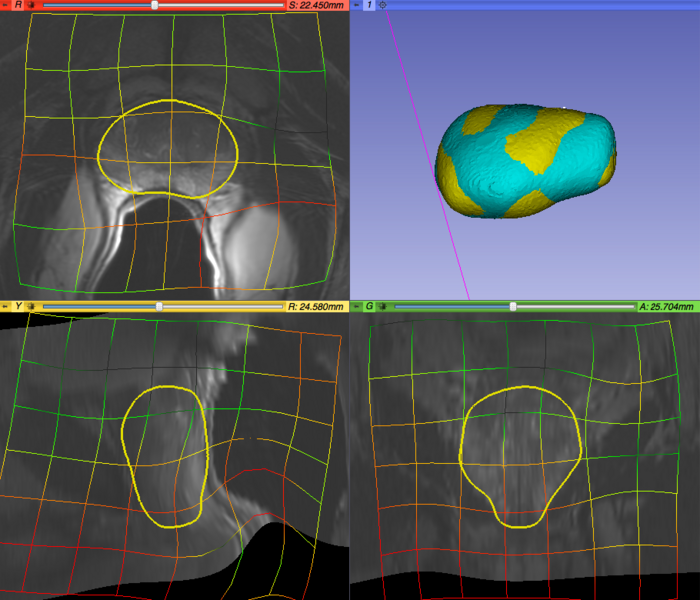
\includegraphics[width=10cm]{1_intro/img/MapBasedRegistration.png}
      \caption{Example of registration for MR images}
    \end{figure}

    他にも、臓器などの動き追跡のために用いられることがある。
    例えば、Fuら\cite{fu2011motion}はヒト下腿部のMR画像から、運動の追跡とひずみマップを作成した。
    また、Raghavendraら\cite{chandrashekara2003construction}はPCAも組み合わせ、心臓の運動を追跡するモデルを構築した。
    \begin{figure}[ht]
      \centering
      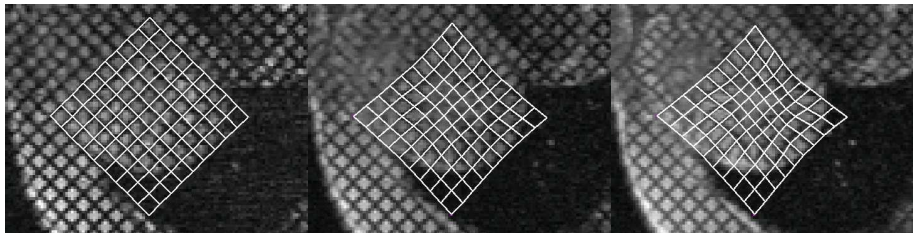
\includegraphics[width=14cm]{1_intro/img/heart_registration.png}
      \caption{A virtual tag grid used in registration for motion tracking of mid-ventricular short-axis slices\cite{chandrashekara2003construction}.}
    \end{figure}

    また、レジストレーションは放射線治療にも用いられている\cite{velec2011effect}。
    呼吸運動と線量蓄積の影響を変形画像レジストレーションを用いることで検討することが可能となり、正確なレジストレーションが可能となることにより、腫瘍および正常組織の線量の変化を定量化することができる。

    上記の通り、画像レジストレーション技術の発展に寄与することは医療の質や効率の向上だけでなく、医師の負担軽減にも繋がるため、非常に重要である。

\subsection{画像モダリティ}
    医療画像には様々なモダリティが存在する。
    医療分野においてモダリティとは、医療機器の種類やタイプを指す言葉であり、代表的なモダリティにはMRIやX線などが挙げられる。
    このモダリティのうち、一種類のみを用いてレジストレーションを行う場合、それをモノモーダルレジストレーション(monomodal registration)と呼ぶ。

    モノモーダルレジストレーションと異なり、2つまたはそれ以上の複数モダリティを対象に行われるレジストレーションはマルチモーダルレジストレーション(multimodal registration)と呼ばれる。
    多くの場合、異なる2つのモダリティから得られる画像は、補完的な性質を持つ。
    先程例に上げたMR-TRUSは、解像度とリアルタイム性を2つのモダリティによって補完し合っている。

    今日、モノモーダルレジストレーションの多くは高い精度で自動化され、実際に臨床でも利用され始めている。
    しかし、マルチモーダルレジストレーションにおいては、利用することの利点は明らかであるにも関わらず、診断臨床の現場ではほとんど行われていない\cite{viergever2016survey}。

\subsection{問題点}
    治療法の選択および治療計画の術前段階でのマルチモーダルレジストレーションは普及しているものの、自動化の研究は進んでいない。
    これには様々な理由が存在しているが、主な理由は以下に挙げる3点である。

    \subsubsection{レジストレーション対象および手法の多様性}
        自動レジストレーションの主な問題の一つに、その種類の豊富さが挙げられる。
        本項では、いくつかの例を挙げてその複雑性について論ずる。
    \begin{description}
        \item[次元数]\mbox{}\\
            まず、空間的な次元のバリエーションである。
            医療画像には2D平面だけでなく、3Dのボクセルを扱う場合がある。
            つまり、医療画像レジストレーションでは、少なくとも2D同士、2D-3D、3D 同士のレジストレーションの3種類が存在する。
            2-D-2-Dレジストレーションは、パラメータの数とデータ量の両方の複雑さがはるかに少ないので、多くの場合、3-D-3-Dの場合よりも簡単かつ迅速にレジストレーションすることが可能である。
            2-D-2-Dレジストレーションは、パラメータの数とデータ量が非常に少ないため、多くの場合、3-D-3-Dの場合よりも簡単かつ迅速にレジストレーションを行うことが可能である。
    
            また、空間的次元とは異なり、時系列を表す意味での次元が考慮される場合がある。
            例えば小児における骨の成長モニタリング\cite{saeed1998magnetic}などでは時系列的に同一患者の画像を比較することが求められる。
            さらに、このような時系列的な比較では空間的次元と同様にその間隔によってレジストレーションの難易度が変化する。
            高頻度で撮像を行えばレジストレーションはより容易になるが、逆に撮像の間隔が長い、または変化が早い場合にはレジストレーションの難易度は高くなる。
            

        \item[モダリティ]\mbox{}\\
            モダリティの多さも、レジストレーションの複雑性を増す原因となる。
            画像モダリティは、2つのカテゴリーに大別することができる。
            \begin{figure}[ht]
              \centering
              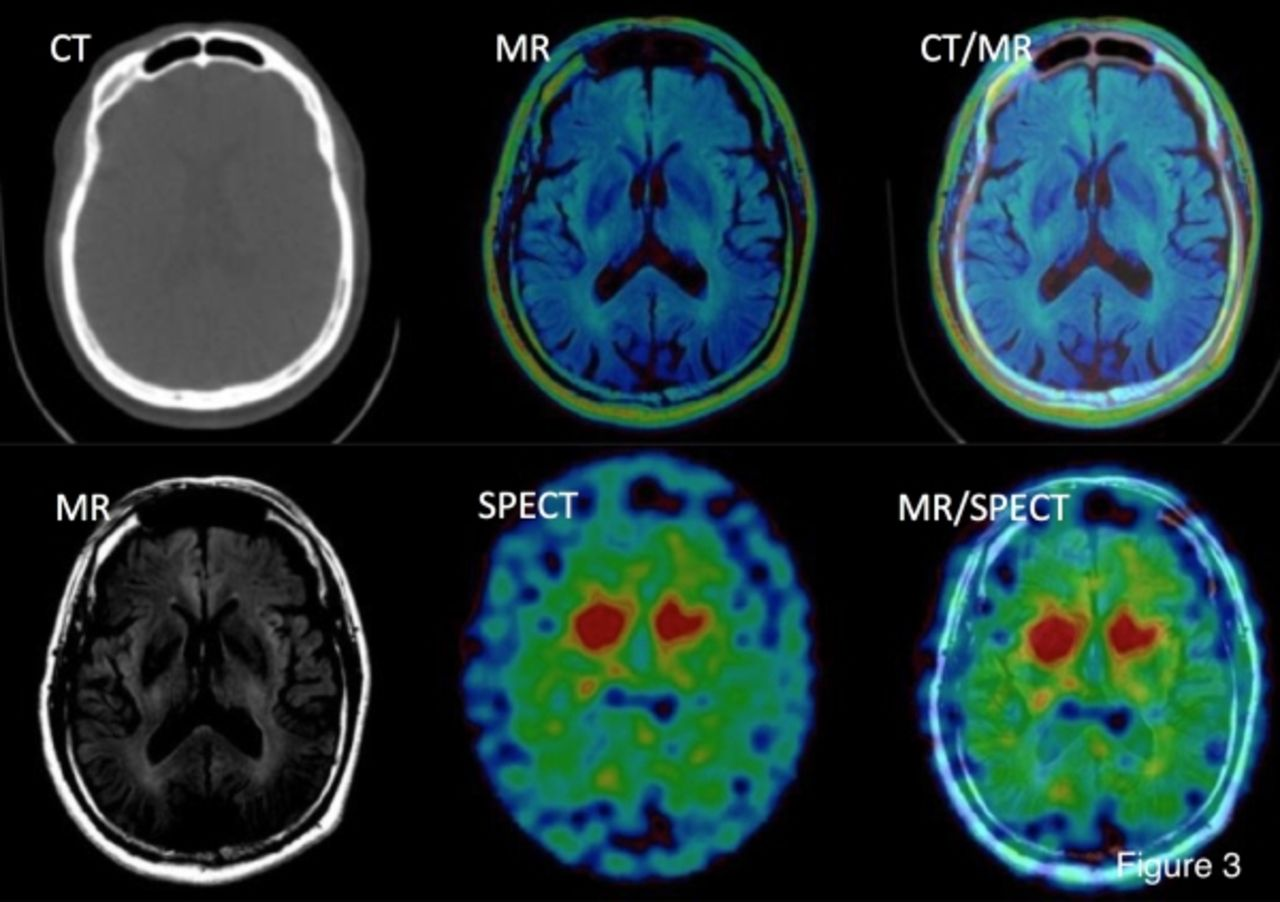
\includegraphics[width=12cm]{1_intro/img/MRCTSPECT.jpg}
              \caption{Brain cross-section images in various modality\cite{hara2016spect}.}
            \end{figure}
            一つは解剖学的モダリティであり、CT(Computed Tomography)、MRI(Magnetic Resonance Imaging)、X-ray、US(Ultrasound)などが存在し、その中でも、MRIなどはT1, T2などの細かい分類が存在する\cite{maintz1998survey}。
            もう一つは機能的モダリティであり、このモダリティは代謝に関する情報を主に描画する。
            例えばSPECT(single photon emission CT:単光子放出型コンピュータ断層撮影法)や、PET(Positron Emission Tomography : 陽電子放出断層撮影法)、fMRI(functional magnetic resonance imaging)などが挙げられる。
            他にも脳波などのような空間的に疎な技術も機能的画像技術と呼ぶことが可能であるが、一部を除きいた機能的モダリティの画像のほとんどが、レジストレーションには活用されない。
    
            このように、画像モダリティは非常に多様であり、またそれぞれのモダリティで特性が異なるため、すべてのモダリティで同時に動作する手法を開発することは困難を極める。
            さらに、異なるモダリティ同士のレジストレーションを行う、マルチモーダルレジストレーションの場合には、2つの画像を比較することすら困難であり、レジストレーションの難易度は飛躍的に高くなる。
            このようにモダリティの差異がレジストレーションにもたらす複雑性は特筆すべきものであるが、その程度は様々である。
            例えば、MR画像におけるT1,T2画像の差と、MR-US画像の差では、後者の差が前者と比べて非常に大きいことがわかる。
    
            また、モダリティの違いがもたらす複雑性は画像の外観だけに留まらない。
            撮像している機材が異なるということは、撮像する機器ごとに、撮像範囲、撮像するタイミング、患者の姿勢などが異なることになる。
            撮像範囲が異なる場合、比べる画像ごとに写っている臓器の数が異なることになる。
            また、撮像するタイミングが異なることによって、膀胱などの時間によって大きさが変化するような臓器への対応が困難になる。
            さらに、MRIやCTのように、体軸に沿って一定間隔ずつの画像しか撮像不可能な場合、完全に同じ断面を撮像することは困難である。
            加えて、患者の姿勢によって臓器の相対位置や断面方向に差が生じる可能性も考えられる。

        \item[変形手法]\mbox{}\\
            変形手法の多さも、レジストレーションの複雑性を増す原因となる。
            画像の変形手法には様々な方法が存在する。
            まず、変形対象の画像をパッチに分けてそれぞれを変形するパッチベースの手法と、画像全体を変形する手法に大別される。
            そして、具体的な変形手法として剛体変換、アフィン変換、透視変換、そして非線形変換と、4つの手法が存在する。
            \begin{figure}[ht]
              \centering
              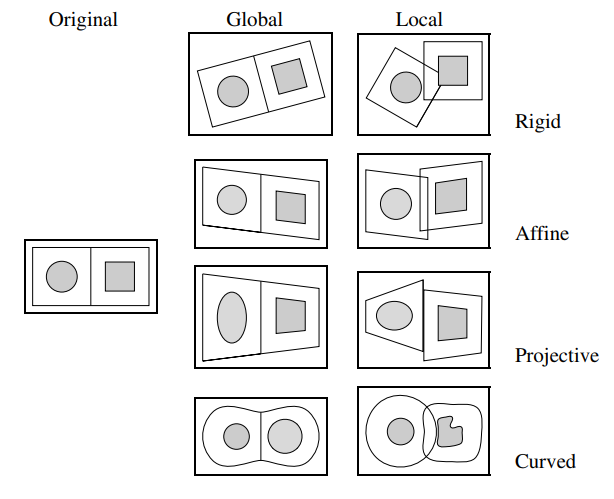
\includegraphics[width=10cm]{1_intro/img/2Dtransformations.png}
              \caption{Examples of 2-D transformations\cite{maintz1998survey}.}
            \end{figure}
    
            中でも非線形変換の方法は多岐に渡り、数式で一般的に表現することはない。
            非線形変換を用いた画像変形方法の一例としては、TPS(Thin Plate Spline)変換などが存在する。
            また、画像レジストレーションでも特にDIR(Deformable image registration)においては、displacement vector field (DVF)を用いた画像の変換が行われることが多い。
            これは非線形変換の一つであり、移動画像の各画素を対象画像の対応する画素位置に移動させるための変位ベクトル場(DVF)を生成することにより、移動画像を対象画像に合わせて変形させる技術である。
            
            以上のような多様な画像変形手法の中から、各研究が様々な手法を採用しており、定量的評価を行うのは困難を極めている。
            また、現在臨床現場に導入されているほとんどが最も簡単な剛体変換のみを採用している\cite{viergever2016survey}。
    \end{description}


    \subsubsection{データの欠如}
        データの欠如に関しても医療画像レジストレーションの自動化を妨げる大きな要因の一つである。
        % ref 2016 a survey of medical image registrations -under review
        医療画像レジストレーションに関するデータセット整備の必要性は度々指摘されており、深層学習が自動画像レジストレーションの研究に広く利用されるようになって以降、その傾向は顕著である。
        % ref deep learning in medical image registration: a review
        
        例えば、
    
    \subsubsection{検証の困難さ}
        医用画像レジストレーションの精度評価は非常に複雑で複雑である。
        この原因はこれまでに述べた2つの
        % ref 1998 survey of medical image registrations
        % ref 2016 a survey of medical image registrations -under review

\subsection{主な手法}
    画像レジストレーションの手法は,様々な角度から分類が可能である\cite{maintz1998survey}。
    例えば、画像レジストレーションを行うために患者の身体にマーカーを埋め込む侵襲的な手法\cite{lunsford2012modern, van1995automatic}と、そうでない手法で大別することが可能である。
    他には、レジストレーションの基準に何を用いるか(ランドマーク基準\cite{evans1996correlative, uenohara1995vision}、セグメンテーション基準\cite{zhao1993registration, andersson1995method}、ボクセル値基準)によって大別することも可能である。
    しかし、現在ではほとんどのレジストレーション操作が非侵襲的で、画像の比較にはボクセル(またはピクセル)を利用するようになった。

    現在用いられている主な手法は2つに大別される。
    類似度を最大化するように変形を繰り返す反復的手法と、変形パラメータを直接導出するパラメータ推定手法である。
    本節ではこの2つの分類に沿って、いくつかの医療画像レジストレーション手法を示す。
    
    \begin{figure}[ht]
      \centering
      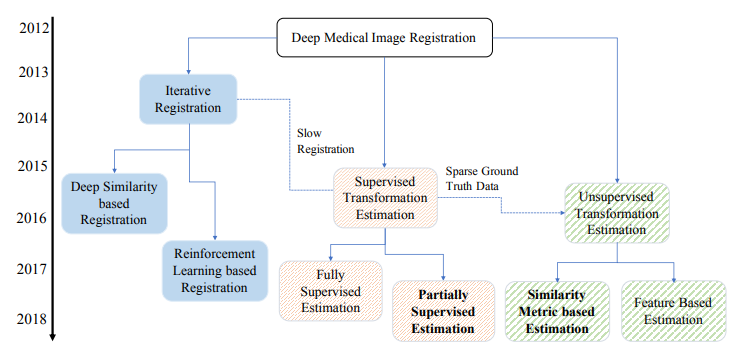
\includegraphics[width=14cm]{1_intro/img/classification_of_method.png}
      \caption{An overview of deep learning based medical image registration broken down by approach type. The popular research directions are written in bold.\cite{haskins2020deep}.}
    \end{figure}
    
    \subsubsection{反復的手法}
    
    \subsubsection{教師あり学習}
    
    \subsubsection{半教師あり学習}
    
    \subsubsection{教師なし学習}
    
    \subsubsection{敵対的学習}

    % TODO
    % 画像レジストレーションの主な手法
    % 反復的手法
    % パラメータ推定法
    % 医療画像レジストレーションの問題点
    % データの欠如
    % 検証の困難さ

\section{ドメイン適応}
    % TODO
    % ドメイン適応の分類
    % ドメイン適応の医療応用
    % 医療画像レジストレーションにおけるドメイン適応活用の現状
    \subsection{分類}
\subsection{医療応用}
\subsection{医療画像レジストレーションにおけるドメイン適応活用の現状}

\section{研究目的}
    % TODO
    \subsection{既存技術の問題点}

\subsection{課題設定}
    モダリティ間の外観差は入力データ分布の差であると捉えることができる.
    ドメイン適応(Domain Adaptation, DA)は入力データの分布の差に対処するための技術であり,医療画像においてはMultimodal Segmentationなどのタスクに応用されている.
    Multimodal Registrationに対してDAを用いる手法はいくつか存在するものの,Single Step Registrationに適用されている例は非常に少ない.

\subsection{貢献}
    本論文では、DAを用いることで,Registrationの教師データを用いることなくMultimodal Registrationが可能なモデルを訓練する手法を提案する.
    本論文で我々は自然画像で訓練されたRegistration modelの性能が、DAを用いることによってどのように変化するかを観察することにより,DAの医療画像Registrationへ応用可能性を示す.

\section{論文構成}
    この論文は次のように構成される.
    第1章は序論であり,本研究の背景並びにその目的について述べた.
    第2章は本研究の位置付けを明らかにするものであり,関連する研究について述べる.
    第3章はドメインの違いを確認する操作および、ドメイン適応を利用しない場合におけるマルチモーダル画像レジストレーションに関する実験の結果と考察について述べる.
    第4章では提案手法によるドメイン適応およびマルチモーダル画像レジストレーションの結果と考察について述べる.
    第5章では本研究に対する結論を述べる.